\section{SEGA}
Originally short for \textit{Service Games} and officially styled as SEGA, is a
Japanese multinational video game developer and publisher headquartered in
Tokyo, Japan, with multiple offices around the world. Sega developed and
manufactured numerous home video game consoles from 1983 to 2001, but the
financial losses incurred from its Dreamcast console caused the company to
restructure in 2001\cite{SEGA}.


\subsection{Sega Genesis:}
The Sega Genesis, known as the Mega Drive in most regions outside of North
America, is a 16-bit home video game console which was developed and sold by
Sega Enterprises, Ltd. The Genesis was Sega's third console and the successor
to the Master System. Sega first released the console as the Mega Drive in
Japan in 1988, followed by a North American debut under the Genesis moniker
in 1989\cite{SegaGenesis}.\\
According to the data the Sega Genesis only released 29 games with sales for
\$30.78 million dollars, its most representative game is \textit{Sonic the
  Hedgehog 2} released in 1992 by SEGA itself with sales of \$6.03 million dollars.

\subsection{Sega CD:}
The Sega CD, released as the Mega-CD in most regions outside North America,
is a CD-ROM accessory for the Sega Genesis video game console designed and
produced by Sega as part of the fourth generation of video game consoles. The
add-on was released on December 12, 1991 in Japan, October 15, 1992 in North
America, and 1993 in Europe. The Sega CD lets the user play CD-based games
and adds extra hardware functionality, such as a faster central processing
unit and graphic enhancements\cite{SegaCD}. With total sales of \$1.87 millions
and 6 released games according to the dataset; is the 2nd lowest performing
platform of SEGA. The most representative title for this platform is
\textit{Sonic CD} with \$1.5 million dollars (more than half of the whole
platform sales) released in 1993.

\subsection{Sega Saturn:}
The Sega Saturn is a 32-bit fifth-generation home
video game console that was developed by Sega and released on November 22,
1994 in Japan, May 11, 1995 in North America, and July 8, 1995 in Europe as
the successor to the successful Sega Genesis. The Saturn has a dual-CPU
architecture and a total of eight processors. Its games are in CD-ROM format,
and its game library contains several arcade ports as well as original
titles\cite{SegaSaturn}.\\
This platform contains 173 registered games according to the data with total
sales of \$33.59 million dollars; the most representative game is
\textit{Virtua Fighter 2} released in 1995 with \$1.93 million dollars in
sales.

\subsection{Sega Gamegear:}
The Game Gear is an 8-bit handheld game console released by Sega on October
6, 1990 in Japan, 1991 in North America and Europe, and Australia in
1992. The Game Gear primarily competed with Nintendo's Game Boy, the Atari
Lynx and NEC's TurboExpress. The handheld shares much of its hardware with
the Master System and is able to play its own titles as well as those of the
Master System, the latter being made possible by the use of an
adapter. Containing a full-color backlit screen with a landscape format, Sega
positioned the Game Gear as a technologically superior handheld to the Game
Boy\cite{SegaGameGear}. The only game available from the dataset is
\textit{Sonic The Hedgehog 2 (8-bit)} with sales only in Japan for \$0.04
million dollars.

\subsection{Sega Dreamcast:}
The Dreamcast is a home video game console released by Sega on November 27,
1998 in Japan, September 9, 1999 in North America, and October 14, 1999 in
Europe. It was the first in the sixth generation of video game consoles,
preceding Sony's PlayStation 2, Nintendo's GameCube and Microsoft's Xbox. The
Dreamcast was Sega's final home console, marking the end of the company's 18
years in the console market\cite{SegaDreamcast}. With global sales for
\$15.97 million dollars and 52 registered games is the 3rd worst performing
platform according to the dataset. Its most notorious game is \textit{Sonic
  Adventure} released in 1998 with sales for \$2.42 million dollars.\\

To see with more detail SEGA's sales across the different platforms, point
\textit{ARMeet} to Figure \ref{fig:SegaImage.}\\

\begin{figure}[h]
  \centering
  \centerline{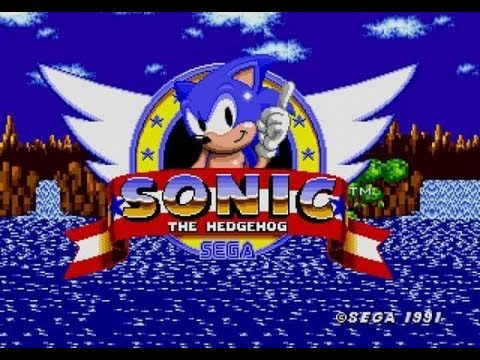
\includegraphics[scale=0.8]{images/SegaMainTarget.png}}
  \caption{Representative picture of SEGA, point ARMeet to this image to
    see the different sales on each platform.}
  \label{fig:SegaImage}
\end{figure}

%% Sega
%% Platforms: 5
%% Platform: SEGA_GENESIS
%% Games: 29
%% Total Sales: 30.78, by country US: 21.05 EU: 6.05 JP: 2.699999 Other: 0.97

%% Platform: SEGA_GAMEGEAR
%% Games: 1
%% Total Sales: 0.04, by country US: 0 EU: 0 JP: 0.04 Other: 0

%% Platform: SEGA_CD
%% Games: 6
%% Total Sales: 1.87, by country US: 1 EU: 0.36 JP: 0.45 Other: 0.05

%% Platform: SEGA_SATURN
%% Games: 173
%% Total Sales: 33.59001, by country US: 0.72 EU: 0.54 JP: 32.26001 Other: 0.06999999

%% Platform: SEGA_DREAMCAST
%% Games: 52
%% Total Sales: 15.97, by country US: 5.43 EU: 1.69 JP: 8.560001 Other: 0.27
